% !TeX program = xelatex
% !TeX encoding = UTF-8
\documentclass{MathorCupmodeling}
\usepackage{amsmath}
\usepackage{ctex}
\usepackage{booktabs}
\bianhao{MC2303283}
\tihao{A}
\timu{基于QUBO模型与退火算法的信用评分卡组合优化问题求解}
\keyword{QUBO模型;量子退火;模拟退火;信用评分卡;组合优化;整数规划模型}
\begin{document}
	\begin{abstract}
本文根据金融信贷的实际问题,进行数学建模为整数规划模型,针对评分卡的组合优化信用问题,本文运用了量子退火等多种方法,充分发挥了物理学中量子理论的思想在优化问题上的优势,根据题意构建\textbf{QUBO}模型,并借助 python 的 pyqubo、neal 等工具包编程求解。
  
        问题一中,要求在100个信用评分卡中找出1张及其对应的阈值,使最终收入最多,针对该问题进行建模并将模型转为\textbf{QUBO}形式进行求解。本文先对原问题进行了化简操作,根据题目建立更加常见的0-1规划模型,再通过一系列证明和程序验证,将模型进行\textbf{QUBO}建模,在拉格朗日乘数的选择上,我们通过多次程序验证给出了较优的结果,并且在接下来的问题求解中,我们都与传统的求解方法进行了正确性验证。
        
       问题二中,要求给赛题数据中的信用评分卡1、 信用评分卡2、信用评分卡3这三种规则设置其对应的阈值,使最终收入最多,针对该问题进行建模并将模型转为\textbf{QUBO}形式进行求解。与第一问不同的是,这一问的通过率涉及到了累乘,我们提出了一些处理0-1变量累乘的方法,如考虑取对数指数转换为累加,考虑使用一个因子函数替代决策变量。此种思想具有一般性,一样可以适用于第三问。对于Q矩阵的建立,我们发现所建立的目标函数是三维的,直接求解较为困难,因此提出了一种与惩罚函数类似的引入拉格朗日乘数的方法进行降维。
       
        问题三中,要求从所给附录中100个信用评分卡中任选3种信用评分卡并设置合理的阈值,使得最终收入最多,针对该问题进行建模并将模型转为\textbf{QUBO}形式进行求解。这个问题与第二问类似,但是阶数更高,并且在传统计算机中已经难以得出结论。我们沿用第二问的结论构造模型,并提出了引入辅助函数化简累乘的方法,最后使用了量子退火进行求解,与常见的模拟退火算法进行比较验证。最终模型有着比较好的计算结果,给出了三种相对最优的方案可供参考。

最后,对本文所涉及的方法进行评价总结,我们认为模型的可优化空间非常大,虽然相对之前的传统模型有着比较好的优势,但是仍存在很多待解决的优化问题。同时量子计算有着很好的前景,在实际生活中可以解决多种问题,本文研究的内容对实际应用也有一定的参考意义。
	\end{abstract}
	\tableofcontents\newpage
	\section{问题重述}
	\subsection{问题背景}
   在银行信用卡或相关的贷款等业务中,对客户授信之前,需要先通过各种审核规则对客户的信用等级进行评定,通过评定后的客户才能获得信用或贷款资格。规则审核过程实际是经过一重或者多重组合规则后对客户进行打分,这些规则就被称为信用评分卡。
   
  每个信用评分卡有多种阈值设置,但只有一个阈值生效,这就使得不同的信用评分卡在不同的阈值下,对应不同的通过率和坏账率,一般通过率越高,坏账率也会越高,反之,通过率越低,坏账率也越低。对银行来说,通过率越高,通过贷款资格审核的客户数量就越多,相应的银行获得的利息收入就会越多,但高通过率一般对应着高坏账率,而坏账意味着资金的损失风险。选择不同的信用评分卡,不同的阈值组合,会给银行带来不同的收入与损失,由此决定银行最终收入。由于银行场景的复杂性,往往需要采用选择多个不同的信用评分卡进行组合来实现最佳的风险控制策略。因此,银行的目标是选择最合理的信用评分卡组合以及其阈值,使得银行最终收入最多。
  
  该问题所涉及的组合优化领域是优化领域中最重要的领域之一,在每个行业都有实际应用,也是运筹学、计算机科学和分析学最活跃的研究领域之一。传统方法是由分析师开发一种适合当前问题数学结构的求解算法,虽然这种算法在某些问题环境中产生了良好效果,但实践中出现的应用程序的多样性需要创建多种解决方案技术,每种技术在其最初预期用途之外的应用程序都很有限$^{[1]}$。目前,利用量子计算原理解决优化问题的前景尤其光明$^{[2][3][4][5][6]}$,而QUBO 模型是量子计算的基础,将QUBO模型运行在量子计算机硬件上,可以进行毫秒级的加速求解,这种模型和加速方式在未来各行业中将得到广泛的实际应用。
 	\subsection{问题提出}
  问题1:
在 100 个信用评分卡中找出1张及其对应阈值,使最终收入最多,针对该问题进行建模,将该模型转为 QUBO 形式并求解。

问题2:
假设赛题说明 3 目前已经选定了数据集中给出的信用评分卡1、信用评分卡2、信用评分卡3这三种规则,如何设置其对应的阈值,使最终收入最多,针对该问题进行建模,将模型转为 QUBO 形式并求解。

问题3:
从所给附录中100个信用评分卡中任选取3种信用评分卡,并设置合理的阈值,使得最终收入最多,针对该问题进行建模,并将模型转为 QUBO 形式并求解。

	\section{问题分析}
 数据分析:
 
 对所给定的阈值数据集,通过简单的验证,可以总结出以下特征:
 \begin{enumerate}
     \item 数据无缺失值、异常值
     \item 通过率和坏账率均随着阈值增大而增大
     \item 通过率均为两位小数,坏账率均为三位小数
 \end{enumerate}
  
  问题一中,可以进行数学建模,将通过率、坏账率都通过符号表示,并且表达出收入函数作为目标函数。根据约束条件:限制只能选一张卡一个阈值,可以建立整数规划模型,再将其转化为QUBO模型。

    问题二中,我们需要选择三张银行卡,在实际问题中,银行对客户进行授信的场景非常复杂,往往受到多种因素的影响。根据题意,我们可以将授信流程进行简化。题设要求将坏账率设为三种阈值的坏账率平均,通过率设置为三种通过率相乘。我们可以据此构建新的模型。

    问题三中,解空间相比前两问变大了许多,通过穷举已经难以得出结果。于是我们通过传统模拟退火来验证解的正确性,并通过量子退火求解问题。
 \section{模型假设}
 \begin{enumerate}
      \item 假设银行在贷款流程中的贷款资金为定值M=1000000,银行贷款利息收入为定值r=0.08\%,不受其他因素影响。
 
     \item 假设信用评分卡有100种,每张卡有10种阈值,最多只能对一张卡选择设置一个阈值。

     \item 假设最终收入仅因为信用卡阈值选择进行波动,不考虑其他意外得失的可能性。
\end{enumerate}
 \section{符号说明}
 \begin{center}
 \begin{tabular}{cc}
   \toprule
   符号 & 说明  \\
   \midrule
   M & 贷款资金,题设为1000000元  \\
   r & 利息收入率,题设为0.08  \\
   i & 信用评分卡的编号,取值1到100\\
   j & 阈值的编号,取值1到10\\
   $x_{ij}$ & 0或1,表示信用评分卡i阈值j是否被选择\\
   $x$ & $x_{ij}$组成的列向量\\
   $t_{ij}$ & 信用评分卡i选择j阈值时的通过率 \\
   $h_{ij}$ & 信用评分卡i选择j阈值时的坏账率 \\
   T & 所有信用评分卡通过率组成的矩阵\\
   H & 所有信用评分卡通过率组成的矩阵\\
   Q & QUBO模型中的Q矩阵,为对称阵\\
   \bottomrule
\end{tabular}
\end{center}
	\section{问题一的模型建立与求解}
 \subsection{模型准备}
 QUBO模型:QUBO模型:QUBO模型即二次无约束二进制优化模型。QUBO模型可以包含工业、科学和政府中发现的各种特殊的重要优化问题。正如Kochenberger等人(2014)和Anthony等人(2017)等研究所记录那样,通过易于应用的特殊重新配方技术,一旦将QUBO求解器放入QUBO框架中,就可以利用它们的力量有效地解决许多重要问题。QUBO模型已经成为量子退火这一量子计算领域的基础,并已经成为神经形态计算的一个研究课题$^{[1]}$。
 
 QUBO即二次无约束二值优化模型,形如$max:x^{T}Qx$。其中x是0和1组成的列向量,Q是一个对称矩阵。QUBO模型的基本特征是二值化,也就是说自变量只能取值0和1,以及无约束条件,可以通过增加罚函数的方法,将传统规划模型的约束条件转化为无约束问题.

 也可以将QUBO模型展开,形如:
 $$
 \begin{aligned}
     max: \sum_{i=1}^{n}x_{i}w_{i}+\sum_{j=1}^{n}\sum_{i=1}^{n}x_{j}x_{i}w_{i}w_{j}
 \end{aligned}
 $$

  整数规划模型:在整数规划中,如果所有变量都限制为整数,则称为纯整数规划。如果仅一部分变量限制为整数,则称为混合整数规划。整数规划的一种特殊情形是0-1规划,它的变数仅限于0或1。组合最优化通常都可表述为整数规划问题。两者都是在有限个可供选择的方案中,寻找满足一定约束的最好方案。有许多典型的问题反映整数规划的广泛背景。例如,背袋(或装载)问题、固定费用问题、和探险队问题(组合学的对集问题)、有效探险队问题(组合学的覆盖问题)、旅行推销员问题, 车辆路径问题等。因此整数规划的应用范围也是极其广泛的。它不仅在工业和工程设计和科学研究方面有许多应用,而且在计算机设计、系统可靠性、编码和经济分析等方面也有新的应用。
  
 \subsection{基本整数规划模型的建立}
选定的信用评分卡为 $i(1 \le i \le 100)$,阈值设置为$j(1\le  j \le 10)$,$h_{ij}$对应i卡j阈值坏账率,$t_{ij}$对应i卡j阈值通过率,总坏账率h,总通过率t。T、H代表通过率、坏账率组成的矩阵。  
贷款资金M,利息收入r,卡总数$i_{max} =100$,阈值总数$j_{max}=10$  

根据题目假设,M=100000,r=0.08为常量。
有以下关系式:

收入:$Mrt(1-h)$   
损失:$Mth$  

最终收入:
\begin{equation*}
\begin{aligned}
Mrt(1-h)-Mth &= Mrt-Mrth-Mth \\
&= Mt(r-rh-h) \\
&= Mt[r-(1+r)h] \\
&= Mrt[1-\frac{1+r}{r}h] \\
\end{aligned}
\end{equation*}

由题意,M、r为常数。由于在问题中常数项取值对最大值的$i,j$不影响,可省略部分常数,将题目简化为:求收益函数$f(t,h)=t(1-ah) $ 的最大值,其中$a= \frac{1+r}{r}$为给定值。 

针对问题1,由符号假设,$t_{ij}\in T,h_{ij}\in H.$因此原问题目标函数是关于$T,H,X$的函数。  

定义函数决策变量$x_{ij}\in\{1,0\}$,其中$x_{ij}$组成向量$x$。  

$g_{ij} = f_{ij}x_{ij} = f(t_{ij},h_{ij})x_{ij}$,
目标函数$G=\sum_{i=1}^{100}\sum_{j=1}^{10}g_{ij}$ ,

可针对原问题建立优化模型如下:
$$
max: G(T,H,x)=\sum_{i=1}^{100}\sum_{j=1}^{10}x_{ij}f(t_{ij},h_{ij}) \\
$$
\begin{gather}
s.t.
\left\{
\begin{aligned}
\sum_{j=1}^{10}x_{ij} \le1  &&&&&&{(1-1)} \\
\sum_{i=1}^{100}\sum_{j=1}^{10}x_{ij} = 1  &&&&&&{(1-2)} \\
\end{aligned}
\right.
\end{gather} 

其中,
$$
x_{ij}=
\left\{
    \begin{aligned}
    0,  &&&\mbox{第i卡第j阈值未被选中}\\
    1,  &&&\mbox{第i卡第j阈值被选中}\\
    \end{aligned}
\right.
$$

式(1-1)表示每个卡最多可取一个阈值,(1-2)表示100张卡中有一个阈值被选择。显然,(1-2)条件包含了(1-1)的情况,也就是说约束条件可以省略(1-1).
\subsection{QUBO模型建立}
因为$x_{ij}$是0-1变量,所以$\forall i,j,\mbox{有}x_{ij}^{2}=x_{ij} .$  
$$
\begin{aligned}
g_{ij}= x_{ij}f(t_{ij},h_{ij})  = x_{ij}^{2}f(t_{ij},h_{ij}),\\ 
G=\sum_{i=1}^{100}\sum_{j=1}^{10}x_{ij}^{2}f(t_{ij},h_{ij})&&&&&(1-3)\\
\end{aligned}
$$
  
这是一个组合优化问题。可通过以下步骤,将目标函数转化为QUBO形式.
\begin{enumerate}
\item 
$x_{ij}$组成$100\times 10=1000$维的一元列向量$x=(0,\dots,1,\dots,0)$,可将编号$i,j$进行降维处理至$x_{k}(1\le k \le 1000)$即只使用一个值对$x$的约束,相关的转化方式为:
$$
i = \lceil \frac{k}{10}\rceil \\
$$
\begin{gather}
\left\{
\begin{aligned}
j = 1&&&\cdots \mbox{k是10的倍数}\\
j=k &\mod  10 &&\cdots \mbox{k不是10的倍数}\\
\end{aligned}
\right.
\end{gather}
\item
通过查阅文献知道,根据约束条件可定义惩罚函数,将问题转化为无约束优化。
$$
\begin{aligned}
penalty = -P(\sum_{k=1}^{1000}x_{k} -1)^{2}
\end{aligned}
$$
其中,P为一个相对目标函数可能取值的一个极大的数,若不满足约束条件,惩罚函数会极大地减小函数值,避免此解被选中为最优解,因此对目标函数起到约束作用。  
\item
矩阵$Q=(f_{k})_{1000}=(f_{ij})_{1000}$,由于(1-3)只包含$x_{ij}$相关的平方项,因此在引入罚函数前,Q矩阵是一个$1000\times1000$的对角阵,$Q_{k} = f(t_{k},h_{k})=t_{k}(1-ah_{k}).$  

综上所述,可对原优化问题进行初步QUBO建模:
$$
\begin{aligned}
max:x^{T}Qx-P(\sum_{i=1}^{1000}x_{k} -1)^{2}\\
=\sum_{i=1}^{1000}t_{i}(1-ah_{i})x_{i}-P(\sum_{i=1}^{1000}x_{k} -1)^{2}\\
\end{aligned}
$$
将罚函数与Q矩阵合并,$Q=diag(t_{1}(1-ah_{1}),t_{2}(1-ah_{2}),\dots,t_{1000}(1-ah_{1000}))-PE_{1000}.$,E代表一个1000阶全为1的矩阵。

Q矩阵是QUBO对目标函数的建模中最为重要的一点,在之后的求解过程中,我们可以将难以转化成标准QUBO形式的目标函数,通过pyqubo封装的{compiled\_qubo.to\_qubo()[0]}功能辅助转换QUBO模型,得到Q矩阵,其结果也符合我们的推导猜想。可以参考附录2返回值。


\item
罚系数P的选取。P也可以看做是拉格朗日乘数,是一个自由度较高可以自己定义的常数,P值的选取是否合理将直接影响到优化问题是否满足约束条件。在此题中要保证选择唯一阈值时目标函数最大,选择2、3,或更多时结果更小,因此需要满足:在其他多种阈值被选择的情况下,$x^{T}Qx$的作用再大也不大过唯一阈值的情况。这个问题可以通过数学的方式去求解,在这里我们通过多次试验的方式来确定P值的合适范围。

通常来说,P值越大对应的约束条件越强,但可能因此影响结果无法收敛到最优情况。
\end{enumerate}
\subsection{求解与验证}
由于此问题中仅存在1000个可能的变量,可以通过传统计算机进行循环穷举求解。

结果为:
 \begin{center}
 \begin{tabular}{ccc}
   \toprule
   信用评分卡号 & 阈值选择 & 收入  \\
   \midrule
   49 & 1 & 61172.0 \\
    \bottomrule
   \end{tabular}
   \end{center}
   借助pyqubo的工具包可以直接求解QUBO模型,编写的代码详见附录1。需要注意的是,编码时以计算机习惯从0开始计数,所以得到的k值结果与上述(2)式相差1,计算的结果是x[480],也就是k=481,即i=49,j=1,与穷举法结果一致。

   在此问题中,经过多次试验,我们将拉格朗日乘数选在个位数这个数量级。因为启发式算法每次运行结果可能不同,会在接近最优解处局部收敛,我们通过多次的程序运行,总结了程序得到的结果与惩罚函数的关系,并在此基础上对模型进行改进。

   当P=5时,12次运行所得的解集为$\{(720,58.51519),(201,57.2276),(480,61.1719),\\
   (480,61.17199),
   (481,61.02159),(431,55.5212),(480,61.171),(480,61.171),(130,55.14),\\
   (480,61.17199),(250,56.0),(481,61.1719)\}$
   可见其实能正确得到精确结果的情况较少,多数是在接近最优的点附近。
      \begin{figure}[ht]
  \centering
  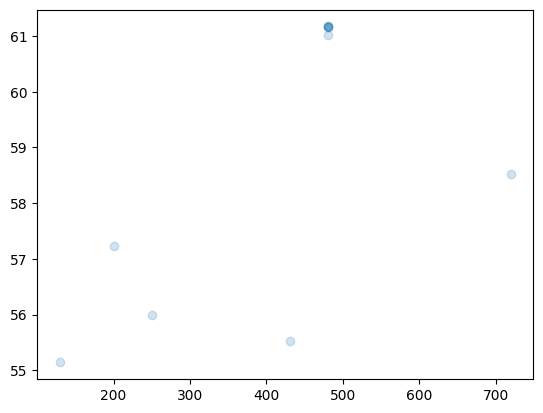
\includegraphics{figure/output.png}
  \caption{算法多次运行结果}
  \label{fig:my_label}
\end{figure}
 	\section{问题二的模型建立与求解}
  \subsection{规划模型建立}
  与问题一不同的是,这一问需要选择三个信用卡的阈值组合。根据题意,对选中的i阈值,通过率$t=\prod_{i=1}^{3}t_{i}$,坏账率$h=\frac{1}{3}\sum_{i=1}^{3}h_{i}$,
  
  沿用问题一推导得到的收入函数$f(t,h)=t(1-ah) $,决策变量$x_{ij}$,可以初步建立以下规划模型:
  $$
max: f(t,h) \\
$$
\begin{gather}
s.t.
\left\{
\begin{aligned}
\sum_{j=1}^{10}x_{1j} =1   \\
\sum_{j=2}^{10}x_{2j} =1   \\
\sum_{j=3}^{10}x_{3j} =1 \\
\end{aligned}
\right.
\end{gather} 
(3)式中约束条件代表信用评分卡1、2、3分别有且仅可选择1个阈值。
但是,值得注意的是,由于决策变量$x_{ij}$可能取值为0,所以我们不能直接像处理累加那样,将$x_{ij}t_{ij}$直接相乘,这样的结果会恒为0,这也是这个问题最为棘手的一点。经过一系列的思考,我们提出了一些处理累乘的建模思路。
\subsection{累乘的建模处理}
\subsubsection{转化为指数形式}
\begin{enumerate}
    \item 对T矩阵各个值取对数,对下标i,j降维至k后,T为30维对角矩阵。
        $T=diag(t_{1},t_{2},\dots,t_{30})$,得到的$T' = diag(ln(t_{1}),ln(t_{2}),\dots,ln(t_{30}))$
    \item $x^{T}T'=(\dots,ln(t_{k_{1}}),\dots,ln(t_{k_{2}}),\dots,ln(t_{k_{3}})\dots))$\\
    $x^{T}Tx =ln(t_{k_{1}})+ln(t_{k_{2}})+ln(t_{k_{3}})$,其中$k_{1},k_{2},k_{3}$是选择的阈值。此时我们已经可以得到乘积,因为$ln(t_{k_{1}})+ln(t_{k_{2}})+ln(t_{k_{3}})=ln(t_{k_{1}}t_{k_{2}}t_{k_{3}})$,只需要再将其转为指数幂函数即可。
    \item 对上述式子求指数,我们可以得到$t=e^{x^{T}T'x}=t_{k_{1}}t_{k_{2}}t_{k_{3}}$
\end{enumerate}
目标函数可以表示为$max:e^{x^{T}T'x}(1-\frac{a}{3}x^{T}Hx)=e^{\sum_{i=1}^{30}ln(t_{i})x_{i}}(1-\frac{a}{3}\sum_{i=1}^{30}h_{i}x_{i})$

此时只存在累加,但是涉及到指数运算,可能仍然难以转化为QUBO模型。此方法若要进行求解,更加适用于整个目标函数只存在累乘的情况。
\subsubsection{用一种简单加和表示累乘的决策变量}
定义决策变量组成的函数因子$(1-x_{i}+t_{i}x_{i})$,观察到,若$x_{i} = 0$,函数因子取值为1,若$x_{i} = 1$,函数因子取值为$t_{i}$.这个方法非常巧妙地使可以用k从1-30的累乘表达$t_{k_{1}}t_{k_{2}}t_{k_{3}}$。

即:
通过率$t=\prod_{i=1}^{30}(1-x_{i}+t_{i}x_{i})$,目标函数可以表示为:
max:$\prod_{i=1}^{30}(1-x_{i}+t_{i}x_{i})(1-\frac{a}{3}\sum_{i=1}^{30}h_{i}x_{i})$
\subsubsection{三阶降维}
由于这个问题涉及的因子较少,可以尝试将问题变为三次的,再降维到二次。目标函数可表达为:
$max:\sum_{j_{1}}^{10}\sum_{j_{2}}^{10}\sum_{j_{3}}^{10}t_{1j_{1}}t_{2j_{2}}t_{3j_{3}}x_{1j_{1}}x_{2j_{2}}x_{3j_{3}}(1-\frac{a}{3}\sum_{i=1}^{30}h_{i})$
常见的降维方法如:将$x_{1j_{1}}x_{2j_{2}}$乘积表示为一个新的变量t’。
\subsection{建模转换}
我们使用上述方法2的技巧,可以建立模型 
$$
max: G=\prod_{i=1}^{30}(1-x_{i}+t_{i}x_{i})(1-\frac{a}{3}\sum_{i=1}^{30}h_{i}x_{i})
$$
\begin{gather}
s.t.
\left\{
\begin{aligned}
\sum_{j=1}^{10}x_{1j} =1   \\
\sum_{j=2}^{10}x_{2j} =1   \\
\sum_{j=3}^{10}x_{3j} =1 \\
\end{aligned}
\right.
\end{gather} 
为了建立QUBO模型,我们可以先定义罚函数,同样根据第一问的规则进行了下标降维:
$$
\begin{aligned}
penalty = -P(\sum_{j=1}^{10}x_{j} -1)^{2}-P(\sum_{j=11}^{20}x_{j} -1)^{2}-P(\sum_{j=21}^{30}x_{j} -1)^{2}
\end{aligned}
$$
由于此问题只涉及到三种信用评分卡,我们这里结合次数更低的方法3来构造模型,方法2的模型转换可以参考问题三的部分。最终建立的模型为:
$$
\begin{aligned}
max:\sum_{j_{1}=1}^{10}\sum_{j_{2}=1}^{10}\sum_{j_{3}=1}^{10}t_{1j_{1}}t_{1j_{1}}t_{2j_{2}}t_{3j_{3}}x_{1j_{1}}x_{2j_{2}}x_{3j_{3}}(1-\frac{a}{3}\sum_{i=1}^{30}h_{j}x_{j})\\
-P(\sum_{j=1}^{10}x_{j} -1)^{2}-P(\sum_{j=11}^{20}x_{j} -1)^{2}-P(\sum_{j=21}^{30}x_{j} -1)^{2}
\end{aligned}
$$

接下来将介绍降维的方法。

引入一个新变量$y_{i}=x_{1j_{1}}x_{2j_{2}}$,t可表达为:$\sum_{j_{1}=1}^{10}\sum_{j_{2}=1}^{10}\sum_{j_{3}=1}^{10}y_{i}t_{1j_{1}}t_{2j_{2}}t_{3j_{3}}x_{3j_{3}}$,我们发现对下标i,难以表达它的取值范围。于是,参考约束条件惩罚函数的建立,我们定义一个拉格朗日乘数$\lambda$,控制$y_{i}-x_{1j_{1}}x_{2j_{2}}=0$,在此操作后的模型:
\begin{gather}
max:\sum_{j_{1}=1}^{10}\sum_{j_{2}=1}^{10}\sum_{j_{3}=1}^{10}t_{1j_{1}}t_{1j_{1}}t_{2j_{2}}t_{3j_{3}}y_{i}x_{3j_{3}}(1-\frac{a}{3}\sum_{i=1}^{30}h_{j}x_{j})-\lambda(y_{i}-x_{1j_{1}}x_{2j_{2}})^2\\
-P(\sum_{j=1}^{10}x_{j} -1)^{2}-P(\sum_{j=11}^{20}x_{j} -1)^{2}-P(\sum_{j=21}^{30}x_{j} -1)^{2}
\end{gather}
\subsection{求解与验证}
我们通过编写程序进行了QUBO模型的求解,实际上,pyqubo可以直接处理高次项问题,将其转化为二次,并不需要严格的数学证明推导。详细代码可以参见附录2与支撑文件。

此问题中可能的情况数目与上一问相同,也是$10\times10\times10=1000$种可能的组合,因此也可以通过传统计算机进行循环穷举求解,在两种方法对比后,我们得到了精确的答案。

结果为:
 \begin{center}
 \begin{tabular}{ccc}
   \toprule
   信用评分卡号 & 阈值选择 & 总收入  \\
   \midrule
   1 & 8 & 27914.8 \\
   2 & 1 & \\
   3 & 2 & \\
    \bottomrule
   \end{tabular}
   \end{center}
   \section{问题三的模型建立与求解}
   \subsection{模型建立}
   问题三其实和第二问类似,对于我们在上一问建立的模型,有着比较好的一般性,可以直接沿用。
   $$
max:G=\prod_{i=1}^{1000}(1-x_{i}+t_{i}x_{i})(1-\frac{a}{3}\sum_{i=1}^{1000}h_{i}x_{i})
$$
\begin{gather}
s.t.
\left\{
\begin{aligned}
\sum_{j=1}^{10}x_{ij} \le 1   \\
\sum_{i=1}^{100}\sum_{j=1}^{10}x_{ij} =3 \\
\end{aligned}
\right.
\end{gather} 
在QUBO模型建立中,罚函数定义为:
$$
\begin{aligned}
penalty = -P(\sum_{j=1}^{1000}x_{j} -3)^{2}-P(\sum_{j=1}^{10}x_{j}+c_{j} -1)^{2}
\end{aligned}
$$
其中,$c_{j}$为引入的松弛变量,也是0-1变量。

为了得到QUBO模型,我们先处理$\prod_{i=1}^{1000}(1-t_{i}+t_{i}x_{i})$的展开式。对于1000个变量,展开后的多项式将包含$2^{1000}$项,这无疑是非常复杂的。在这个问题中,我们的目标是找到一个简化的形式,以便更容易地构建QUBO矩阵。

我们尝试通过计算几个具体的例子来发现规律,可以将原问题情况个数设为n=1000,$\prod_{i=1}^{n}(1-t_{i}+t_{i}x_{i})$。

当n=1时:
\begin{center}
$t = (1-t_1+t_1x_1)$
\end{center}
当$n = 2$时:
\begin{center}
$(1-t_1+t_1x_1))(1-t_2+t_2x_2)$

$= 1+t_1t_2(x_1-1)(x_2-1)+t_1(x_1-1)+t_2(x_2-1)$
\end{center}
可以看出,当计算更高阶的情况时,展开的过程会变得更加复杂。同时,我们也尝试了在不展开的情况下直接通过近似来处理原始问题。注意到:
\begin{center}
    
$f(x_1, x_2, ..., x_n) = \prod_{i=1}^{n}(1-t_{i}+t_{i}x_{i})(1-\sum_{i=1}^{n}\frac{1}{3}h_{i}x_{i})$

$ = (1-\sum_{i=1}^{n}\frac{1}{3}h_{i}x_{i}) \prod_{i=1}^{n}(1-t_i) \prod_{i=1}^{n}(1-x_iy_i)$
\end{center}
定义两个辅助函数$g$和$h$,它们分别表示$\prod_{i=1}^{n}(1-t_i)$和$\prod_{i=1}^{n}(1-x_it_i)$。因为目标是最小化$f$。将$g$和$h$代入$f$,我们有:
\begin{center}
$f(x_1, x_2, ..., x_n) = (1-\sum_{i=1}^{n}\frac{1}{3}h_{i}x_{i}) gh$
\end{center}
可以将原始问题转化为以下形式:
\begin{center}
$ \max_{x_i \in {0, 1}} (1-\sum_{i=1}^{n}\frac{1}{3}h_{i}x_{i}) gh$
\end{center}

在这种情况下,将问题转化为QUBO需要采取近似方法或者使用启发式算法来求解。以惩罚函数使用的拉格朗日松弛技术为启发,我们可以用相同的方法对问题中的gh进行处理。我们可以将问题转化为一个二次型式,并在求解过程中逐渐调整拉格朗日乘子。

将原始问题的约束条件引入目标函数,使用拉格朗日乘子$\lambda_i$:

$L(x, y, \lambda) = (1-\sum_{i=1}^{n}\frac{1}{3}h_{i}x_{i}) gh + \sum_{i=1}^{n} \lambda_i (y_i - t_i x_i)$

问题的目标为最小化拉格朗日函数$L(x, y, \lambda)$,以此来满足$y_i = t_i x_i$。将$gh$展开为一个关于$x_i$的二次型式,然后将其与拉格朗日项相结合,从而得到一个关于$x_i$和$y_i$的二次型式。

接下来,可以借助编程工具构造QUBO矩阵$Q$,并求解QUBO问题。这个过程可能需要多次迭代,以便逐渐调整拉格朗日乘子$\lambda_i$,使其满足约束条件。

对于较大的$n$,这个问题将变得非常复杂,需要大量的计算资源来求解。在这种情况下,可以考虑结合启发式算法来寻找接近最优解的可行解。这些算法通常不保证找到全局最优解,但它们可以在有限的计算时间内找到一个相对优秀的解。
\subsection{模型求解}
\subsubsection{使用传统模拟退火求解}
由于在这个情况下,可选择的情况一共有$C_{100}^{3}\times10^{3}$次,要进行上亿次计算,在普通的计算机算力下已经很难得出结果。并且,我们可以通过数学证明,证明“选择多张卡进行组合”这个问题的时间复杂度是包含阶乘与指数级的,是NP-hard问题,在选择的卡数量为50时运算难度最大。因此若要得出结果,需要使用优化算法进行验证。我们这里选择了模拟退火与量子退火进行了比较验证。

模拟退火具体的流程可以参考图2.

具体的实现方法:对于161700种可能的卡组合,我们先定义了一个index列表作为索引。
index=[[0, 1, 2],
 [0, 1, 3],
 [0, 1, 4],
 [0, 1, 5],
 [0, 1, 6],
 [0, 1, 7],
 [0, 1, 8],
 [0, 1, 9],\dots]
完整的退火代码详见附录2,在附录的代码中给出了一个简单的测试例。
\begin{figure}[ht]
  \centering
  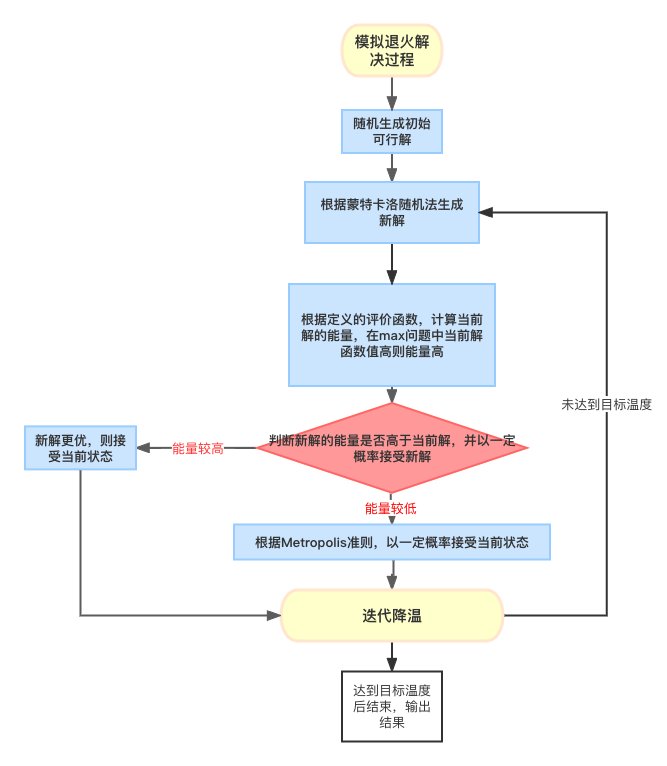
\includegraphics[width= 0.8\linewidth]{figure/sa.png}
  \caption{传统模拟退火流程图}
  \label{fig:my_label}
\end{figure}

图3给出了一次模拟退火的迭代过程,横轴代表迭代次数,纵轴代表评价函数的值。在编写代码中我们将问题转化为了极小值问题,即通过加负号把最大值问题转为最小值,因此所得的迭代图是向下的趋势,在编写程序时为了优先得到最优编号,省略了常数,因此纵轴可能与最优值不匹配。
\begin{figure}[ht]
  \centering
  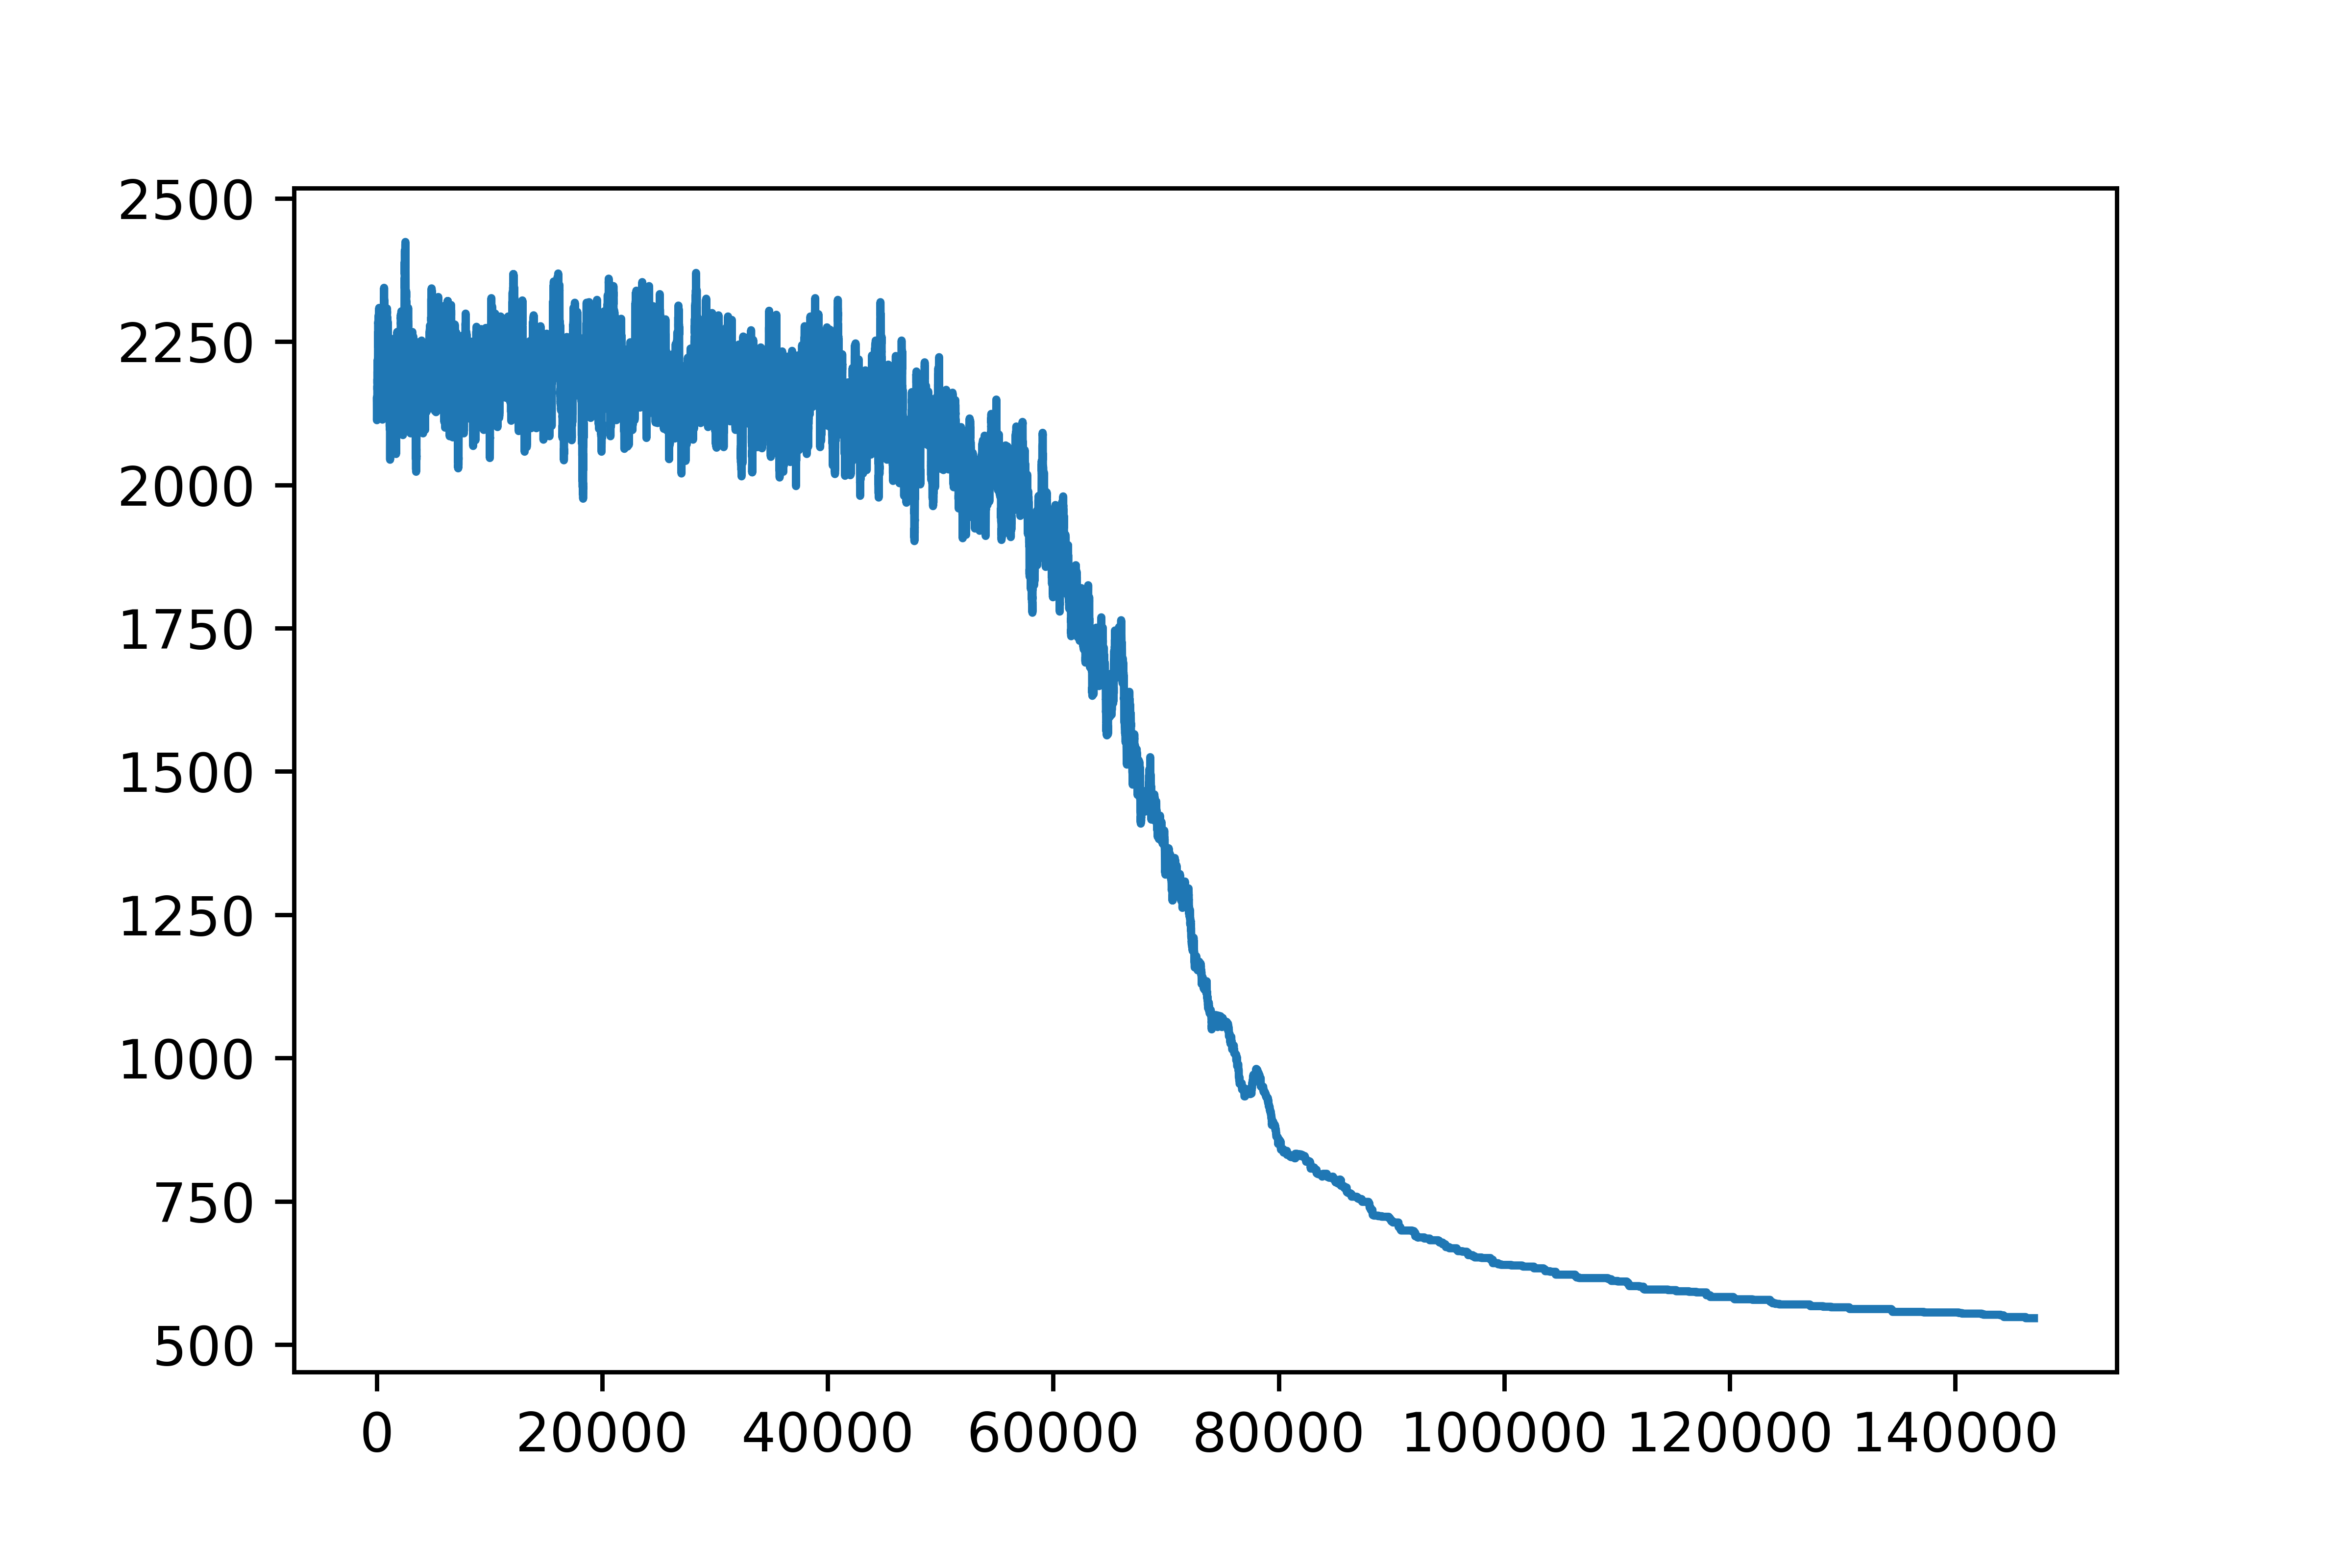
\includegraphics{tsp_sa_evolution.png}
  \caption{模拟退火迭代图}
  \label{fig:my_label}
\end{figure}
\subsubsection{使用量子退火求解}
量子退火:量子计算促进了量子力学原理在计算中的应用,从1982年起量子计算获得了很大的发展势头。目前存在许多量子算法,它们比著名的经典算法运行得更有效。绝热量子计算是由Farhi等人在21世纪初提出的。它基于量子力学的一个重要定理,绝热定理。这个定理断言,如果量子系统是由一个从Hinit进化到Hfin的缓慢变化的哈密顿量驱动的,那么如果系统从Hinit的基态开始,系统将最终处于Hfin的基态。已经证明绝热量子计算等同于标准量子计算。量子退火基于量子绝热计算范式,被用于解决组合优化问题。量子退火器试图解决问题的方式与使用经典模拟退火解决优化问题的方式非常相似。通过多元函数构建能源景观,使得基态对应于问题的解决方案。量子过程被迭代,直到以足够高的概率找到最优解。“量子退火器”中的“量子”是指使用多量子位隧道。高度并行性是量子退火相对于经典代码执行的优势。量子退火器并行探索所有可能的输入,以找到问题的最佳解决方案$^{[7]}$。

与模拟退火算法最大的不同是,量子退火在新解的选取上进行了一定的优化,使用了量子物理里量子隧穿的思想。在模拟退火中,生成新解基于蒙特卡洛模拟,当降温时遇到相对较差的解集合时,模拟退火必须要多次迭代才能跳过。而量子退火引入随机的哈密顿量,使得有一定概率跳过较差解集合,在现有的文献材料中,量子退火有着很明显的效率优势。

在python库neal中,我们可以方便地调用量子退火函数进行求解。我们的求解结果为[71, 325, 482],各对应的值如下表,并且给出了一些相对较优的方案可供参考:
\begin{center}
 \begin{tabular}{cccccccc}
   \toprule
   评分卡号1 & 阈值选择 & 评分卡号2 & 阈值选择 & 评分卡号3& 阈值选择 & 总收入  \\
   \midrule
    8 &2 &33 &6 &49&3 & 43880.9\\
    8 &4 &33 &6 &49&3 & 43853.7\\
8 &4 &33 &6 &49&2 & 43826.6\\
    \bottomrule
   \end{tabular}
   \end{center}
	\section{模型评价与改进}
 \subsection{模型缺点与局限性}
    在这几天的研究中,我们发现QUBO模型和量子退火都是一项很新颖的技术,在解决NP-hard的组合优化问题上大放异彩,这无疑是非常令人振奋的。与此同时,也说明这项技术存在着极大的可优化空间,就现在来说可解决的问题还有一定的局限性。我们总结了一些建模上发现的难点。
    \begin{enumerate}
        \item 如何选择决策变量,QUBO和ising等模型的特点是决策变量只能取二值变量。
        \item 对大规模问题计算速度会较慢,比如问题一的1000维矩阵,实际上计算速度和结果与传统计算机相比是没有优势的。
        \item 如何对目标函数进行QUBO建模,这也是本次数学建模问题中最难最重要的一点,很多时候目标问题并不能直接转化为QUBO所要求的二次函数。
    \end{enumerate}
    针对我们建立的模型,我们认为还存在非常多的不足,第一问中散点图可以看出来收敛效果并不好,很难得到最优解,原因是建立的矩阵维数过高,第三问也是如此。我们建立的模型已经超出了题目的需要,题目只需要三个数相乘,而我们的目标函数也可以表示为更多的数相乘,因此我们认为这并不代表着最优。
    
        对于合适的矩阵维数,我们通过记录程序运行时间和矩阵阶数的关系,可以看出来低阶(100内)的矩阵运行速度是非常快的,这也足够解决大部分的需要。但现实中,就我们处理的金融信贷而言,需要在数以万计的客户中进行抉择,怎么进行建模压缩到低阶矩阵、怎么对高阶矩阵优化运行速度,这些都是可以继续讨论的点,可优化空间非常大。
    \begin{center}
 \begin{tabular}{cccc}
   \toprule
 矩阵阶数 &10 & 100 & 1000  \\
   \midrule
运行时间 & 0.08324s & 2.229s & 3.6910s \\
    \bottomrule
   \end{tabular}
   \end{center}
       \subsection{优化方向}
       通过查阅文献$^{[8]}$,我们了解到一种改进的量子退火方法,这个方法对接受解的方法Metropolis 接受准则进行了改进,引入了物理学中粒子在势场中的透射系数。在同一解空间进行搜索时,可以显著提升程序运行速度,这是一种可行的优化方法。
       此外,我们认为还可以结合其他启发式算法的思想,比如粒子群算法、禁忌搜索等,来改进退火过程,进行量子计算。
	\phantomsection
	\addcontentsline{toc}{section}{参考文献}
	\begin{thebibliography}{99}
	\bibitem{label}Fred Glover, Gary Kochenberger, Yu Du. Quantum Bridge Analytics I: A Tutorial on Formulating and Using QUBO Models[J]. 4OR-Q J Oper Res, 17:335-371, 2019.
 \bibitem{label}Perdomo-Ortiz A, Dickson N, Drew-Brook M, Rose G, Aspuru-Guzik A. Finding low-energy conformations of lattice protein models by quantum annealing[J]. Scinetific Report, 2, 571, 2012.
 \bibitem{label} Sarkar A.Quantum Algorithms: For Pattern-Matching in Genomic Sequences[D]. Technische Universiteit Delft, 2018.
 \bibitem{label}Biamonte J, Wittek P, Pancotti N, Rebentrost P, Wiebe N, Lloyd S.Quantum machine learning[J]. Nature, 549, 195, 2017.
 \bibitem{label}Papalitsas C, Karakostas P, Andronikos T, Sioutas S, Giannakis K. Combinatorial GVNS(General 
Variable Neighborhood Search) Optimization for Dynamic Garbage Collection[J]. Algorithms, 11, 38, 2018.
 \bibitem{label}Rebentrost P, Schuld M, Wossnig L, Petruccione F, Lloyd S. Quantum gradient descent and Newton’s method for constrained polynomial optimization[J]. NewJ.Phys, 21, 073023, 2019.
  \bibitem{label}C Papalitsas, T Andronikos, K Giannakis, G Theocharopoulou, S Fanarioti. A QUBO Model for the Traveling Salesman Problem with Time Windows[J]. Algorithms, 12, 224, 2019.
  \bibitem{label}张洪涛,熊红梅,凃玲英.一种改进的量子退火算法[J].江西师范大学学报(自然科学版),2016.
	\end{thebibliography}

	\newpage
	\appendix
	\ctexset{section={
		format={\zihao{-4}\heiti\raggedright}
	}}
	\begin{center}
		\heiti\zihao{4} 附\hspace{1pc}录
	\end{center}
	\section{QUBO求解源代码}
 问题一:
\begin{python}
import numpy as np
from pyqubo import Array, Constraint, solve_qubo

# 定义二进制变量 x
x = Array.create("x", shape=1000, vartype="BINARY")

# 定义原始目标函数
f = sum(t[i] * (10 - 135 * h[i]) * x[i] for i in range(1000))

# 定义约束条件
constraint = Constraint((sum(x[i] for i in range(1000)) - 1) ** 2, label="constraint")
# 定义拉格朗日乘数
lagrange_multiplier = 10000
# 定义带有约束的目标函数
g = -f + lagrange_multiplier * constraint
# 编译目标函数,生成QUBO
compiled_qubo = g.compile()
# 解决QUBO问题
qubo, offset = compiled_qubo.to_qubo()
solution = solve_qubo(qubo)
# 创建SA求解器
sa = neal.SimulatedAnnealingSampler()
# 采样
sampleset = sa.sample_qubo(qubo)
# 解码
decoded_samples = model.decode_sampleset(sampleset)
best_sample = min(decoded_samples, key=lambda x: x.energy)
# 输出最优解
best_sample.sample
print("解决方案:",solution)

#在结果字典中寻找value为1的键值对
def get_key_by_value(d, target_value):
    for key, value in d.items():
        if value == target_value:
            return key
    return "Value not found in the dictionary"
get_key_by_value(best_sample.sample,1)

\end{python}
问题二:
\begin{python}
import numpy as np
from pyqubo import Array, Constraint, solve_qubo

# 定义参数
a = 5
num_variables = 30

# 定义变量
x = Array.create('x', shape=(num_variables, 10), vartype='BINARY')

# 定义目标函数G
G = np.prod([(1 - x[i] + t[i+1] * x[i]) * (1 - a / 3 * np.sum(h[i+1] * x[i] for i in range(num_variables ))) for i in range( num_variables)])

# 定义约束条件
constraints = [Constraint(np.sum(x[i, j] for j in range(10)) - 1, label=f'constraint_{i}') for i in range(num_variables)]

# 构建QUBO模型
model = G + sum(constraints)
qubo, offset = model.compile().to_qubo()

# 求解QUBO模型
solution = solve_qubo(qubo)

# 解码结果
decoded_solution, broken, energy = model.decode_solution(solution, vartype='BINARY')
print(decoded_solution)

\end{python}
由于篇幅限制,更详细的过程代码请参考支撑材料。
\section{不使用QUBO模型的求解代码}
问题三的索引:
\begin{python}
index = []
for i in range(0,100):
    for j in range(i+1,100):
        for q in range(j+1,100):
            temp =[i,j,q]
            index.append(temp)
index
\end{python}
模拟退火代码:
\begin{python}
import random
import math

def objective_function(index, h, t):
    """
    目标函数,计算 t[i1] * t[i2] * t[i3] * (1 - 13.5 / 3 * (h[i1] + h[i2] + h[i3]))
    """
    i1, i2, i3 = random.choice(index)
    new_index = [i1, i2, i3]
    return t[i1] * t[i2] * t[i3] * (1 - 13.5 / 3 * (h[i1] + h[i2] + h[i3]))

def acceptance_probability(old_cost, new_cost, temperature):
    """
    计算接受概率
    """
    if new_cost > old_cost:
        return 1.0
    else:
        return math.exp((new_cost - old_cost) / temperature)

def simulated_annealing(index, h, t, temperature, cooling_rate, min_temperature, max_iterations):
    """
    模拟退火算法
    """
    current_index = index
    current_cost = objective_function(current_index, h, t)
    best_index = current_index
    best_cost = current_cost
    iteration = 0
    while temperature > min_temperature and iteration < max_iterations:
        # 随机生成新解
        i1, i2, i3 = random.choice(index)
        new_index = (i1, i2, i3)
        new_cost = objective_function(new_index, h, t)

        # 计算接受概率
        ap = acceptance_probability(current_cost, new_cost, temperature)

        # 根据接受概率决定是否接受新解
        if ap > random.random():
            current_index = new_index
            current_cost = new_cost

        # 更新最优解
        if current_cost > best_cost:
            best_index = current_index
            best_cost = current_cost

        # 降温
        temperature *= cooling_rate
        iteration += 1

    return best_index, best_cost

# 示例参数
h = [1, 2, 3, 4, 5]
t = [1, 2, 3, 4, 5]
index = [[0, 1, 2], [1, 2, 3], [2, 3, 4]]
initial_index = random.choice(index)
temperature = 100.0
cooling_rate = 0.95
min_temperature = 1e-8
max_iterations = 1000

# 调用模拟退火算法
best_index, best_cost = simulated_annealing(initial_index, h, t, temperature, cooling_rate, min_temperature, max_iterations)

# 输出结果
print("最优解:", best_index)
print("最优值:", best_cost)
\end{python}
\section{QUBO模型中的Q矩阵}
这是一个返回值示例,展示了pyqubo中通过原目标函数建立QUBO模型的能力。更详细的数据可以通过运行支撑材料的文件来得到。
\begin{python}
{('x[71]', 'x[20]'): 10.0,
 ('x[61]', 'x[16]'): 10.0,
 ('x[97]', 'x[23]'): 10.0,
 ('x[92]', 'x[51]'): 10.0,
 ('x[38]', 'x[30]'): 10.0,
 ('x[56]', 'x[13]'): 10.0,
 ('x[65]', 'x[27]'): 10.0,
 ('x[81]', 'x[20]'): 10.0,
 ('x[4]', 'x[2]'): 10.0,
 ('x[85]', 'x[49]'): 10.0,
 ('x[81]', 'x[10]'): 10.0,
 ('x[24]', 'x[2]'): 10.0,
 ('x[32]', 'x[16]'): 10.0,
 ('x[64]', 'x[64]'): -7.88745,
 ('x[4]', 'x[4]'): -10.3218,
 ('x[72]', 'x[33]'): 10.0,
 ('x[68]', 'x[16]'): 10.0,
 ('x[95]', 'x[2]'): 10.0,
 ('x[99]', 'x[12]'): 10.0,
 ('x[93]', 'x[24]'): 10.0,
 ('x[16]', 'x[4]'): 10.0,
 ('x[79]', 'x[63]'): 10.0,
 ('x[79]', 'x[67]'): 10.0,
 ('x[90]', 'x[42]'): 10.0,
 ('x[55]', 'x[19]'): 10.0,
...
 ('x[86]', 'x[85]'): 10.0,
 ('x[34]', 'x[3]'): 10.0,
 ('x[14]', 'x[11]'): 10.0,
 ('x[77]', 'x[9]'): 10.0,
 ...}
 \end{python}
\end{document}